\documentclass[12]{report}
\usepackage[utf8]{inputenc}
\usepackage[T1]{fontenc}
\usepackage[francais]{babel}
\usepackage{listings}
\usepackage{hyperref} %Pour faire des liens hypertexte dans la table des matières
\usepackage{graphicx}

\hypersetup{ %Paramètres pour les liens hypertextes
	colorlinks=true,
	linktoc=all,
	linkcolor=blue,
}

\lstset{ %Paramètres pour afficher du code
	language=C,
	numbers=left,
	stepnumber=1,
	numbersep=10pt,
	backgroundcolor=\color{white},
	showspaces=false,
	showstringspaces=false,
	showtabs=false,
	tabsize=2,
	captionpos=b,
	breaklines=true,
	breakatwhitespace=true,
	title=\lstname,
}

\title{Projet Technologique : Hashiwokakero} %Titre du pdf
\author{Erwan DUPLAND, Quentin DUART, Adrien JAVEL} %Auteur du pdf
\date\today{} %date de compilation

\begin{document}
\renewcommand{\chaptername}{Partie} %Change le titre des chapitres
\renewcommand{\contentsname}{Sommaire} %Change le titre de la table des matières

\maketitle %Applique le titre défini plus haut
\tableofcontents %Notre table des matières

\part{\underline{Hashiwokakero en mode texte}}
	\chapter{Hashiwokakero V1}
		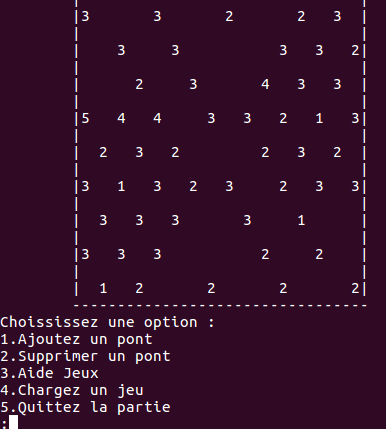
\includegraphics[height=5cm]{hashiwokakeroTEXTE.png} %On affiche l'image hashiwokakeroTEXTE.png
		\section{Les règles originales}
			Le jeu hashiwokakero est un jeu japonais dans lequel il faut relier des \textbf{îles} entre elles.
			Les îles sont numérotées de \textbf{1 à 8} et il ne peut y avoir que 2 ponts au maximum dans une même direction.
			A la fin, le graphe créé par les liaisons entre ces îles doit être connexe et les îles doivent avoir un nombre de
			ponts égal au numéro inscrit sur elles.
		\subsection{game.c}
			Le fichier game.c que nous avons du creer contient pratiquement toutes les fonctions nécessaires au fonctionnement du jeu :
			Création d'une variable de type game, calcul des degrés des nodes, suppression du jeu ainsi qu'une structure game\_s.
			Nous avons cependant rencontrer quelques difficultés dans la mise en oeuvre de ces dernières.
			\lstinputlisting{game.c}
		\subsection{node.c}
			Le fichier node.c est quant à lui, beaucoup plus simple et compact que game.c. En effet, il contient la structure node\_s en elle même :
			\lstinputlisting{node.c}
			De même que les fonctions get\_x et get\_y permettant de récupérer les coordonnées d'une node passée en paramètre, et la fonction get\_required\_degree retournant le degrée de la node souhaitée.
		\subsection{Création de libhashi.a}
			La librairie libhashi.a est une librairie statique créée à partir des fichiers game.c et node.c.
			Elle regroupera donc toutes les fonctions définis dans ces deux fichiers. Par conséquent, au moment de la compilation,
			on utilisera l'option \textbf{-lhashi} pour "linker" la librairie à l'exécutable ainsi généré.

			La ligne de commande pour créer cette librairie est : \fbox{ar rvs libashi.a game.o node.o}

% \lstinputlisting{fichier.c} Affiche le code de fichier.c

	\chapter{Hashiwokakero V2}
		\section{Le caprice du client}
		Maintenant, le client veut que le jeu soit jouable avec de nouvelles règles. Il faut qu'il y ait 8 directions
		(au lieu de 4 dans les règles originales) et que l'on puisse mettre au maximum 4 ponts dans une même direction.
		\subsection{Nouvelle implémentation de game.c}
		Le code de game.c reste globalement le même. Il faut cependant rajouter les directions NE, NW, SE et SW et le fait
		de pouvoir mettre 4 ponts dans une même direction. Le code n'a donc pas beaucoup changé, il a juste été adapté.
	\chapter{Solveur du hashiwokakero}
		\section{Implémentation du solveur}
		Le solveur permettant de résoudre une grille du hashiwokakero est composé de trois fonctions.
		La fonction \textbf{\emph{play\_auto}}.
		La fonction \textbf{\emph{solveur\_recursif}}.
		Et la fonction \textbf{\emph{solveur}}.

		La fonction solveur va appeller la fonction play\_auto et, ensuite, la fonction solveur\_recursif.
		Normalement, si tout se passe bien, le jeu est censé être résolu.

		\subsection{Play auto}
		Play\_auto est une fonction définit dans le fichier hashi\_solve.c. Cette fonction permet de créer les ponts "obligatoires"
		pour pouvoir résoudre le jeu. Il y a donc moins d'opérations effectuées par la fonction solveur\_recursif et on gagne ainsi en rapidité d'éxécution.
		Nous avons par exemple implémenter des coups obligatoires pour des nodes dont le degré est de 8 : On sait déjà qu'il y aura 2 ponts dans chaque direction, ou bien dont le degré est 7 : on ajoute un pont dans chaque direction.
		Nous avons également implémenter différentes techniques issues de IndigoPuzzle.
		\newline \textbf{Just Enough Neighbor Technique} : On test si le noeud possède uniquement 2 voisins
        et si les degrés de ces 2 voisins sont les mêmes que lui, auquel cas on ajoute le nombre de pont requis.
        \newline \textbf{One Unsolved Neighbor Technique}  : On test si le noeud possède exactement un voisin et si son degré est de 1 auquel cas on ajoute immédiatement un pont dans la direction de son voisin.
		\subsection{Solveur récursif}
		La fonction solveur\_recursif est une fonction de type bruteforce. C'est à dire qu'elle va ajouter (si c'est possible)
		des ponts entre deux nodes.
		\newline Étant donné que cette fonction sera appellé après play\_auto, elle fera moins d'opérations que si elle avait été
		apellée avant (car certains node auront déjà tous leur(s) pont(s) ou au moins quelques-uns).
		\subsection{Conclusion sur le solveur}
		Le solveur fonctionne correctement sur les instances \textbf{\emph{game\_default}} et \textbf{\emph{game\_easy}}.
		En revanche, il ne trouve pas de solution pour \textbf{\emph{game\_medium}}.

		Nous avons conclu que ce problème venait de la fonction play\_auto à laquelle nous n'avons pas imposer assez de contraintes.
\part{\underline{Hashiwokakero en interface graphique}}
	\chapter{Hashiwokakero SDL2}
		\section{Le jeu en interface graphique avec la SDL2}
		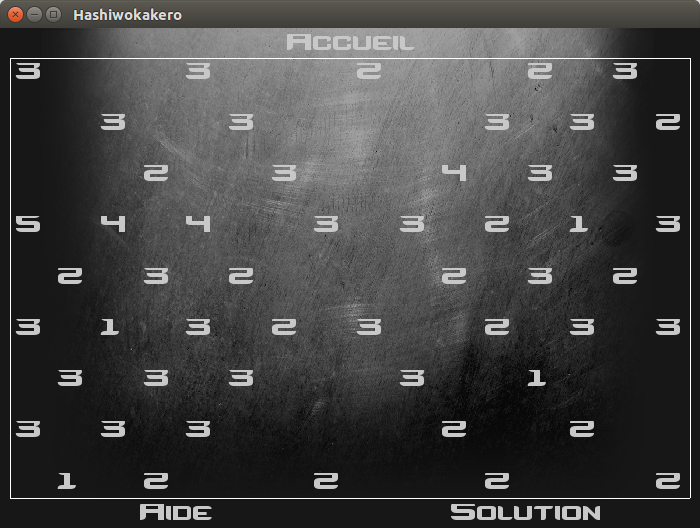
\includegraphics[height=10cm]{hashiwokakeroSDL.png}
		\subsection{Implémentation de l'interface graphique}
                Pour implémenter l'interface graphique, nous nous sommes aidés d'une interface graphique de base. Nous avons donc utilisé trois fonctions \emph{principales} qui utilisent des fonctions \emph{auxiliaires} : \textbf{init}, \textbf{render} et \textbf{process}.

                La fonction \emph{init} permet d'\textbf{initialiser} tous les \textbf{paramètres} stockés dans la structure \emph{env}, la fonction \emph{render} permet de \textbf{placer} dans l'interface graphique les différents \textbf{paramètres} de la structure \emph{env} et la fonction \emph{process} permet d'\textbf{intéragir} avec l'interface avec la \emph{souris} ou avec le \emph{clavier}.

                Nous avons donc créer un \textbf{menu} avec le titre \emph{HASHIWOKAKERO} et les rubriques \emph{Nouvelle partie}, \emph{Règles} et \emph{Quitter}. Si on clique sur la rubrique \textbf{Nouvelle partie}, nous avons un nouveau menu qui arrive avec les rubriques \emph{Facile}, \emph{Moyen} et \emph{Difficile} qui permet de choisir le niveau du jeu. Dès que l'on clique sur un des trois niveau, on arrive sur un nouvel écran avec un \emph{cadre}, la notation \emph{Aide}, la notation \emph{Solution} et la notation \emph{Accueil}.

                La rubrique \textbf{Règles} possède un écran avec, comme son nom l'indique, les \emph{règles} écrites dessus.

                La rubrique \textbf{Quitter} permet de \emph{fermer} l'interface graphique.

                Si nous pouvons améliorer l'interface graphique, nous aurions pu être plus précis dans les zones cliquables en calculant les coordonnées avec précision.


		\subsection{Implémentation du jeu}

		Pour voir la documentation sur notre interface graphique \href{run:documentation.pdf}{cliquez ici} %Lien vers la docu

		L'implémentation du jeu au sein de la SDL n'est pas chose facile : Il a d'abord fallu \emph{afficher chaque noeud} dans un cadre à des coordonnées bien précises.
		Il a également fallu rendre chaque \emph{noeud cliquable}. Pour cela, dans la fonction process, nous avons vérifié que nous cliquions bien entre les coordonnées de chaque noeud. Une fois que deux noeuds sont sélectionnés, si c'est possible, un pont est tracé. En revanche lorsque, entre 2 noeuds, le degré maximal est atteint, les ponts sont supprimés.

		C'est dans la fonction render que nous rendions visibles noeuds et ponts.
\part{\underline{Compilation}}
	\chapter{Compilation}
		\section{Makefile}
		Dans un premier temps, nous avons du réaliser un fichier \textbf{\emph{Makefile}},
		qui est un fichier particulier permettant de compiler rapidement en utilisant la commande : \fbox{make}

		Un Makefile est simplement un fichier dans lequel on définit un ensemble de règles nécessaire à la compilation.
		Par exemple pour compiler un programme s'appellant programme.c et ayant besoin de fichiers include : include1.h et include2.h, on fera :
		\begin{lstlisting}
		programme: programme.c include1.o include2.o
			gcc $^ -o $@
		\end{lstlisting}

		\$\^{} correspond à tous les fichiers après les ":" et \$@ correspond au nom du fichier qui devra être créé, ici : programme.
		\section{cmake}
		Ici, nous avons du créer un fichier \textbf{\emph{CMakeLists.txt}} qui est un fichier dans lequel on définit des règles
		pour créer un Makefile. La syntaxe est un peu plus facile à assimiler et il y a moins de lignes à écrire.
		Pour créer la cible programme à partir de programme.c et des includes include1.h et include2.h, nous ferons ici :
		\begin{lstlisting}
			add_executable(programme programme.c include1.c include2.c)
		\end{lstlisting}
		Pour générer le Makefile il faut alors utiliser la commande \fbox{cmake <répertoire contenant le CMakeLists.txt>}
		Nous n'avons ensuite plus qu'à utiliser la commande \fbox{make} pour compiler le programme.
\end{document}
